\documentclass[12pt]{article}   % you have 10pt, 11pt, or 12pt options

\setlength{\textwidth}{17.2cm}     % if you change this, consider changing
\setlength{\evensidemargin}{-.3cm} % side margins to retain centering
\setlength{\oddsidemargin}{-.3cm}

\setlength{\textheight}{23cm}   % if you change this, consider changing
\setlength{\topmargin}{-2cm}  % top margin to retain centering
\setlength{\headsep}{1.6cm}

%---------------------- These packages below add functionality to your version
%of LaTeX -------------- ---------------------- You might not use all of them
%--------------------------------------
\usepackage[utf8]{inputenc}
\usepackage[T1]{fontenc}
\usepackage{amssymb}
\usepackage{latexsym}
\usepackage{amsthm}
\usepackage{enumerate}
\usepackage{epsfig}
\usepackage{graphicx}
\usepackage{color}
\usepackage{float}
\usepackage{subfig}
\usepackage{amsmath}
\usepackage{makeidx}
\usepackage{fancyhdr}
\pagestyle{fancy}
\usepackage{lastpage}
\usepackage{url}
\usepackage{algorithm}
\usepackage{algorithmic}
\usepackage[algo2e]{algorithm2e}
\usepackage{appendix}
\usepackage{bm}
\usepackage{lmodern} % load a font with all the characters
\usepackage[square, numbers, comma, sort&compress]{natbib}
%------------------------- Customized Header
%--------------------------------------------------------
\fancyhead{}
\fancyfoot{}			
\lhead{Stereo Camera + IMU/INS + GPS}
\rhead{Page \thepage\ of \pageref{LastPage}}

%---------- the symbols below will give you the blackboard bold of R, T, etc.
%----------
\DeclareSymbolFont{AMSb}{U}{msb}{m}{n}
\DeclareMathSymbol{\Sph}{\mathbin}{AMSb}{"53}
\DeclareMathSymbol{\R}{\mathbin}{AMSb}{"52}
\DeclareMathSymbol{\T}{\mathbin}{AMSb}{"54}
\DeclareMathSymbol{\Z}{\mathbin}{AMSb}{"5A}
\DeclareMathSymbol{\K}{\mathbin}{AMSb}{"4B}

%------------------------- Theorem and Proof Environments
%-------------------------------------------------

% This section defines all the environments you might use.  Just type
% \begin{theorem, or corollary, or whatever}, then the optional name of the
% theorem inside {} (or empty {} if no name), then body of the theorem,
% corollary, whatever, also inside {} then \end{theorem, corollary, whatever}
%
% Notice when I use them in the paper, I put an optional "argument" to the
% function and this gives a name to the theorem

\newenvironment{theorem}[1]{\vspace{.9cm}\noindent    {\bf Theorem {#1}}}{\vspace{.1cm}}
\newenvironment{lemma}[1]{\vspace{.9cm}\noindent    {\bf Lemma {#1}}}{\vspace{.1cm}}
\newenvironment{corollary}[1]{\vspace{.9cm}\noindent    {\bf Corollary {#1}}}{\vspace{.1cm}}
\newenvironment{definition}{\vspace{.9cm}\noindent {\bf Definition}}{\vspace{.1cm}}
\def\qed{\hfill $\Box$}
\renewenvironment{proof}{\vspace{.5cm}   \noindent{\bf Proof: }}{\qed \vspace{1cm}}
 
%\theoremstyle{definition} \newtheorem{notation}[theorem]{Notation}
%\newtheorem{properties}[theorem]{Properties}
%\newtheorem{remark}[theorem]{Remark} \newtheorem{example}[theorem]{Example}
%\newtheorem{claim}[theorem]{Claim}
%\newtheorem{observation}[theorem]{Observation}
%\newtheorem{definition}[theorem]{Definition}


% ---------------------- Define case environment ------------------------------

\newcounter{case}

\newenvironment{case}[1]{\stepcounter{case} \addvspace{.5\baselineskip} \noindent\textbf{Case \thecase}. \textit{#1}}{\hfill\fbox{Case \thecase}}

%\newtheorem{case}{Case}
\newtheorem{subcase}{Case}[case] \newtheorem{sub2case}{Case}[subcase]
%\newtheorem{sub3case}{Case}[sub2case] \newtheorem{sub4case}{Case}[sub3case]


%Picture inclusion

\newcommand\pic[3]{
\begin{figure}[H] \begin{center} 
\epsfig{file=#1, height=#2pt} 
\end{center} 
\caption{#3} 
\end{figure}
}

\def\inj{\text{inj}}
\def\diam{\text{diam}}
\def\area{\text{area}}
\def\length{\text{length}}


\begin{document}  % necessary part of document


\title{State Estimation with IMU/INS and camera information}
\author{Zhang Handuo}
\date{\today}

\maketitle

\begin{abstract}
This document is a report on Visual Inertial SLAM using an efficient method of
IMU pre-integration. The pre-integration method combines high frequency IMU data
as a single observation before fusion with camera images, resulting in a much
reduced state and observation graph structure. An accurate map and robot path is
hence obtainable in real-time. We present the pre-integration theory, including
formulation of motion state, observation, uncertainty, observation model and the
Jacobians.
\end{abstract}

\newpage

\tableofcontents

\newpage

\section{Introduction}

\vspace{1cm}
In this work, we firstly introduce a perception system with a set of stereo
camera with IMU. The integration with INS and GPS will be introduced in the next
sections because their formulation is much simpler than that with IMU.
\begin{figure}[ht]
	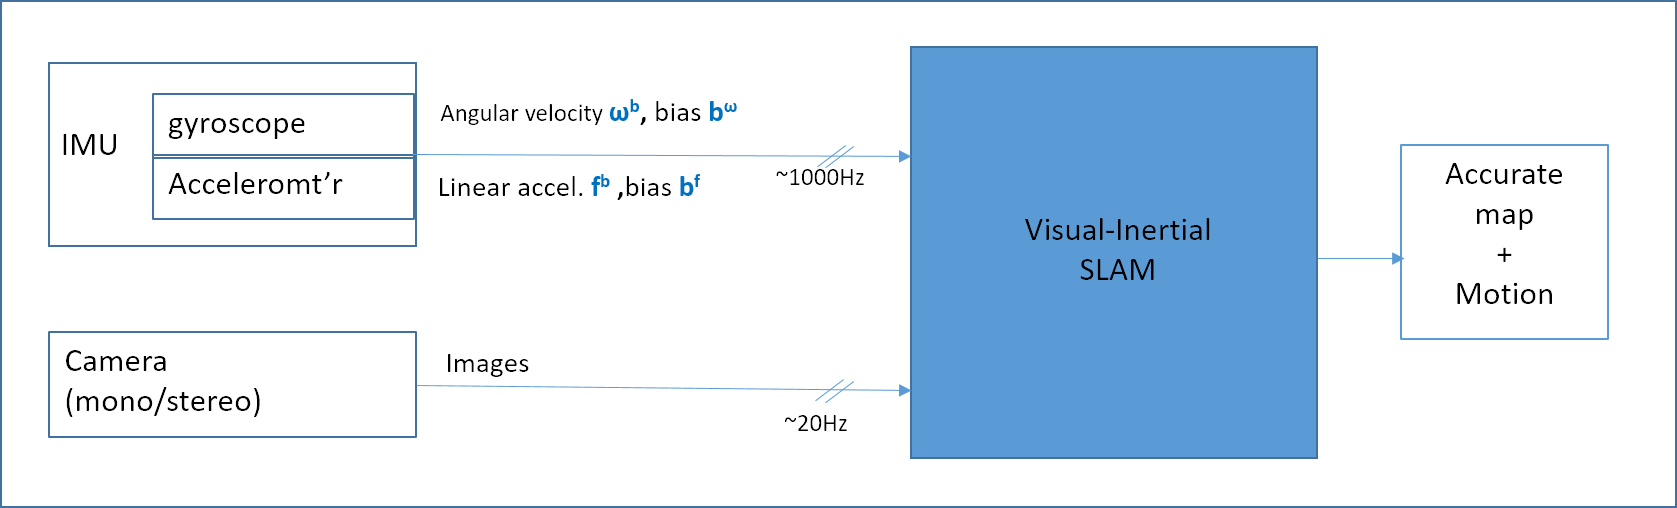
\includegraphics[height=5cm]{figures/VIN_block-diagram.png}
	\caption{Visual Inertial System}
	\label{fig:vin}
\end{figure}

\paragraph{States}
The state vector to be estimated contains the 3-D body position
$\bm{p}^{\mathrm{w}}$, velocity $\bm{v}^{\mathrm{w}}$ and rotations in form of
quaternion $\bm{q}^{\mathrm{w}}$ (converted from raw Euler angles
$\bm{A}^{\mathrm{w}}=[\alpha,\beta,\gamma]$); as well as the M feature locations
($\bm{f}_i^{\mathrm{w}}$) representing visual landmarks where i = 1,...N. 

\paragraph{IMU measurement model}
% The IMU readings include 3-D linear acceleration $\bm{f}^{\mathrm{b}}$ and
% angular rate $\bm{\omega}^{\mathrm{b}}$, both given in body frame and come
% with non-zero bias : $\bm{b}_f$ and $\bm{b}_\omega$. \newline Further, due to
% its design principal, the IMU can only measure acceleration with the gravity
% taken out, therefore the true vehicle's acceleration in the world frame should
% be \\
% $\bm{f}^{\mathrm{w}} = R_b^{\mathrm{w}}( \bm{f}^{\mathrm{b}}-\bm{b}_f ) +
% \bm{g}^{\mathrm{w}}$ \\
For the notation of coordinate transformation and vectors, superscript refers to
the reference frame and here $\{\cdot\}^{\mathrm{w}}$ is the
reference(\textbf{world}) frame. $R_b^{\mathrm{w}}$ and $\Omega_b^{\mathrm{w}}$
are the rotation and angular rate matrices from body frame to world frame,
respectively.


\begin{equation}
	\left\{
	\begin{aligned}
	&\hat{\bm{a}}^b=\bm{a}^b+\bm{b}_a+\bm{R}_w^b\bm{g}^w+\bm{n}_a\\
	&\hat{\bm{\omega}}^b=\bm{\omega}^b+\bm{b}_\omega+\bm{n}_\omega
	\end{aligned}
	\right.
	\label{eq.measurement_model}
\end{equation}
where $\hat{\bm{a}}^b$ and $\hat{\bm{\omega}}^b$ represent the measured
acceleration and angular velocity information of IMU; $\bm{a}^b$ and
$\bm{\omega}^b$ represent true acceleration and angular velocity of the body
itself; $\bm{b}_a$ and $\bm{b}_\omega$ represent the bias of the accelerator and
gyroscope, modeled as the random walk process:
\begin{equation}
\centering
	\left\{
	\begin{aligned}
	&\bm{n}_{\bm{b}_a}\sim\mathcal{N}\left(\bm{0},\bm{\sigma}_{b_a}^2\right),\bm{n}_{\bm{b}_\omega}\sim\mathcal{N}\left(\bm{0},\bm{\sigma}_{b_\omega}^2\right)\\
	&\dot{\bm{b}_a}=\bm{n}_{\bm{b}_a},dot{\bm{b}_\omega}=\bm{n}_{\bm{b}_\omega}
	\end{aligned}
	\right.
	\label{eq.error_model}
\end{equation}
where $\bm{R}_w^b$ is the coordinate rotation matrix from world coordinate to
ego-body coordinate; $\bm{g}^w$ is the gravity acceleration vector under world
coordinate; $\bm{n}_a\sim\mathcal{N}\left(\bm{0},\bm{\sigma}_a^2\right)$ and
$\bm{n}_\omega\sim\left(\bm{0},\bm{\sigma}_\omega^2\right)$ are the Gaussian
white noise of the IMU sensor.
	

\paragraph{Naive visual inertial model}

The motion model based on IMU reading can be stated as
\begin{align}
\begin{split}
	\textrm{time difference:}  \qquad \triangle t & =  t_{t+1} - t_t \\
	\textrm{acceleration:} 	   \qquad \bm{a}_t^{\mathrm{w}} & = R_{bt}^{\mathrm{w}}  (\bm{a}_t^{\mathrm{b}} - \bm{b}_a) \\
	\textrm{velocity:}         \qquad \quad \bm{v}_{t+1} & = \bm{v}_{t} + \bm{a}_t^{\mathrm{w}} \triangle t + \bm{g}^{\mathrm{w}} \triangle t \\
	\textrm{position:}         \qquad \quad \bm{p}_{t+1} & = \bm{p}_{t} + \bm{v}_t \triangle t + \bm{a}_t^{\mathrm{w}} \triangle t^2\\
	\textrm{rotation:}         \qquad \quad \bm{q}_{t+1} & = \bm{q}_t \otimes  \Omega_{bt}^{\mathrm{w}}  (\hat{\bm{\omega}}^b_t - \bm{b}_\omega) \triangle t
\end{split}
\label{eq.motion_model}
\end{align}

\section{The original VI problem}
For a system composed of an IMU and stereo camera navigating with $N$ camera
poses, $K$ IMU samples per image and $M$ features, the naive VI problem includes
robot poses at all IMU sample times.

\paragraph{State Vector}
the state vector $\textbf{X}$ is defined as:
\begin{align*}
\textbf{x} = &(\overbrace{\textbf{q}_{10}, \textbf{p}_{10}, \textbf{q}_{20}, \textbf{p}_{20},... ,\textbf{p}_{K-1,0}, \textbf{p}_{K-1,0},\textbf{q}_{0,1}, \textbf{p}_{0,1},...,\textbf{q}_{K-1,1}, \textbf{p}_{K-1,1},... \textbf{q}_{K-1,N-1}, \textbf{p}_{K-1,N-1},\textbf{q}_{0N}, \textbf{p}_{0N}}^{K \times (N - 1) \ {\mathrm{ poses}}},\\
	 &\overbrace{\textbf{F}_{1},\textbf{F}_{2}, ..., \textbf{F}_{M}}^{M \ {\mathrm{ features}}},\\
	 &\overbrace{\textbf{v}_{00},\textbf{v}_{10} ...,\textbf{v}_{K-1,0}, ...,\textbf{v}_{0,N-1},...,\textbf{v}_{K-1,N-1}, \textbf{v}_{0N}}^{(K \times (N-1)+1)  \ {\mathrm{ velocities}}},\\
	 &\textbf{g}^{\mathrm{n}}, \textbf{A}_{u2c}, \textbf{T}_{u2c}, \textbf{b}_f, \textbf{b}_w )^{\mathrm{T}} 
	 \label{eq.state_vector}
\end{align*}

\paragraph{Observation Vector}
The Observation vector $\textbf{Z}$ is defined as:

\begin{align*}
\begin{split}
\textbf{z}_{raw} &= (\textbf{z}_{camera}, \textbf{z}_{IMUraw}, \textbf{z}_{Tv})' \nonumber \\
=& (\overbrace{\textbf{uv}_{11}, \textbf{uv}_{21}, ... , \textbf{uv}_{M1}, ..., \textbf{uv}_{1N}, \textbf{uv}_{2N}, ... , \textbf{uv}_{MN}}^{M \times N \ {\mathrm{pixels}}}, \nonumber \\ 
& \overbrace{\omega\textbf{f}_{01}, \omega\textbf{f}_{11}, ... , \omega\textbf{f}_{(K-1)1}, ..., \omega\textbf{f}_{0(N-1)}, \omega\textbf{f}_{1(N-1)}, ... , \omega\textbf{f}_{(K-1)(N-1)}}^{K \times (N-1) \ {\mathrm{IMU \ readings}}}, \\
& \overbrace{\textbf{0}, \textbf{0}, ... , \textbf{0}}^{K \times (N-1)  \ {\mathrm{ zero \ contraints}}})^{\mathrm{T}}
\end{split}
% \label{eq.observation_vector}
\end{align*}

% See Appendix \ref{apn:naiveVin} for details on Naive VI motion model and
% optimization details. 
Clearly, such a large state space quickly becomes difficult to manage in
practice. Further, each step of re-linearization, the integration from
acceleration to velocity then to position has to be recomputed, which brings
lots of additional time.

\section{The Preintegration algorithm}

\begin{figure}[!h]
	\begin{center}\begin{tabular}{cc}
		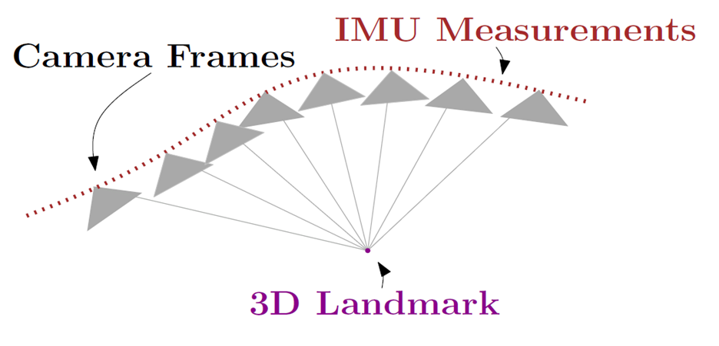
\includegraphics[height=3.3cm]{figures/IMU-sample_Image-frames_3D_illustration.png}&
		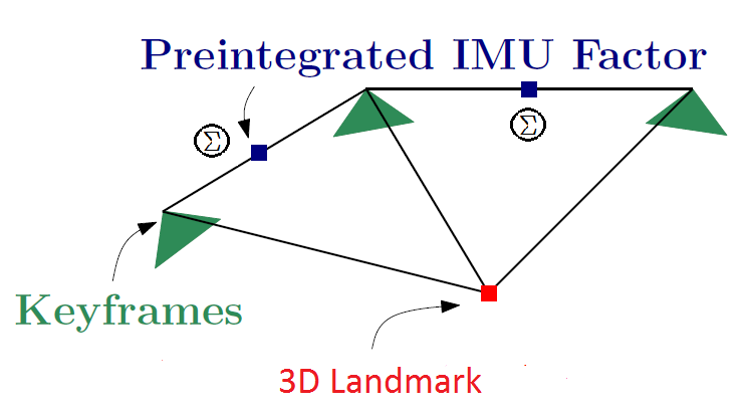
\includegraphics[height=3.3cm]{figures/Preintegrated-IMU_image_3D_illustration.png}\\
		(a) & (b) \\
	\end{tabular}\end{center}
	\caption{(a) Camera+IMU (b) Inertial-delta: preintegrated information \cite{Manifold2015}} 
	\label{fig:VIN sensor information}
\end{figure} 

Todd Lupton first proposed the Preintegration method in 2012 \cite{Lupton2012}:
integrate a large number of high rate IMU observations into a single
observation, making it faster and easier to deal with in a SLAM filter. IMU data
is integrated in a body fixed frame that moves with the vehicle, transformation
to reference frame only happens at the end of integration, hence the algorithm
is referred to as \textbf{Pre-Integration}.

The reference frame in Preintegration visual inertial system is defined as the
body frame at initial robot pose, instead of the traditional globally referenced
frame, preventing the need to reintegrate the state dynamics at each
optimization step.

%With a stereo camera, Todd Lupton also provided a way to recover the absolute
%global frame after 3 images of observation. However this is not possible with
%monocular camera setup.
\subsection{Formulation of Preintegration}
For time consecutive frames $b_k$ and $b_{k+1}$, there exists several
measurements in the time inverval $[t_k, t_{k+1}]$. Given the bias estimation,
we integrate them in the \textbf{local frame} $b_K$ as:

\begin{equation}
\centering
\left\{
\begin{aligned}
&\bm{p}_{b_{k+1}}^{b_k}=\iint_{t\in\left[t_k,t_{k+1}\right]}\bm{R}_{t}^{b_k}\left(\hat{\bm{a}}_{t}-\bm{b}_{a_t}\right)dt^2\\
&\bm{v}_{b_{k+1}}^{b_k}=\int_{t\in\left[t_k,t_{k+1}\right]}\bm{R}_{t}^{b_k}\left(\hat{\bm{a}}_{t}-\bm{b}_{a_t}\right)dt \\
&\bm{q}_{b_{k+1}}^{b_k}=\int_{t\in\left[t_k,t_{k+1}\right]}\frac{1}{2}\bm{\Omega}\left(\hat{\bm{\omega}}_t-\bm{b}_{\omega_t}\right)\bm{q}_t^{b_k}dt
\end{aligned}
\right.
\label{eq.preintegration}
\end{equation}
where $\bm{p}$, $\bm{v}$ and $\bm{q}$ are respectively the
incremental preintegration items for position, velocity and rotation (quaternion
form). Here 

\begin{equation}
\bm{\Omega}\left( \omega \right) = 
\begin{bmatrix}
	- \lfloor \omega \rfloor _ \times & \omega \\
	- \omega ^{\mathrm{T}} & 0
\end{bmatrix}, \lfloor \omega \rfloor _ \times = 
\begin{bmatrix}
	0 & - \omega_z & \omega_y \\
	- \omega_z & 0 & - \omega_x \\
	- \omega_y & \omega_x & 0
\end{bmatrix}.
\label{eq.rot_incremental}
\end{equation}

The details can be found in Appendix (TODO).


\subsection{Bias Correctioin of Incremental preintegration (Continuous Form)}

If the estimation of bias changes minorly, we adjust $\bm{p}_{b_{k+1}}^{b_k}$, $\bm{v}_{b_{k+1}}^{b_k}$, and $\bm{q}_{b_{k+1}}^{b_k}$ by their first-order approximations with respect to the bias as

\begin{equation}
\left\{
\begin{aligned}
&\bm{p}_{b_{k+1}}^{b_k}\approx\hat{\bm{p}}_{b_{k+1}}^{b_k}+\bm{J}^{\bm{p}}_{\bm{b}_{ak}}\delta\bm{b}_a+\bm{J}^{\bm{p}}_{\bm{b}_\omega}\delta\bm{b}_{\omega_k} \\
&\bm{v}_{b_{k+1}}^{b_k}\approx\hat{\bm{v}}_{b_{k+1}}^{b_k}+\bm{J}^{\bm{v}}_{\bm{b}_{ak}}\delta\bm{b}_a+\bm{J}^{\bm{v}}_{\bm{b}_\omega}\delta\bm{b}_{\omega_k} \\
&\bm{q}_{b_{k+1}}^{b_k}\approx\hat{\bm{q}}_{b_{k+1}}^{b_k}\otimes 
	\begin{bmatrix}
		1 \\ \frac{1}{2}\bm{J}^{\bm{q}}_{\bm{b}_{\omega_k}}\delta\bm{b}_{\omega_k}
	\end{bmatrix}.
%\bm{J}^{\bm{q}}_{\bm{b}_{\omega_k}}\delta\bm{b}_{\omega_k}
\end{aligned}
\right.
\label{eq.bias_correction}
\end{equation}

Otherwise if the estimation of bias changes significantly, which far away from the linearization point, we have to do re-propagation under the new bias estimation. So we do not have to propagate IMU measurements repeatedly which save a lot of computational resources.

% \begin{algorithm}
% 	\caption{The Pre-integration Method Based on Inertial Raw Data}
% 	\label{algm:preint}		
% 	\begin{algorithmic}
% 	\STATE Inertial-delta observation $ \triangle \bm{\mathrm{I}} =
% 		\begin{bmatrix} \triangle \textbf{p}_{t}^+ \\ \triangle \textbf{v}_{t}
% 		\\ \triangle \textbf{A} _{t} \end{bmatrix}$, initially set to
% 		$\begin{bmatrix} 0 \\ 0 \\ 0 \end{bmatrix}$ \FOR{$t_1 < t < t_2$} \STATE
% 		$\triangle t =  t_{t+1} - t_t$ \STATE $\textbf{f}_t^{\mathrm{bt1}} =
% 		R_{\mathrm{bt}}^{\mathrm{bt1}} (\textbf{f}_t^{\mathrm{b}} -
% 		\textbf{b}_f)$ \STATE $\triangle \textbf{v}_{t+1} = \triangle
% 		\textbf{v}_{t} + \textbf{f}_t^{\mathrm{bt1}} \triangle t$ \STATE
% 		$\triangle \textbf{p}_{t+1}^+ = \triangle \textbf{p}_{t}^+ + \triangle
% 		\textbf{v}_t \triangle t$ \STATE $\triangle \textbf{A} _{t+1} =
% 		\triangle \textbf{A} _{t} + E_{\mathrm{bt}}^{\mathrm{bt1}} (\omega
% 		_t^{\mathrm{b}} - \textbf{b}_\omega) \triangle t$ \ENDFOR
% 	\end{algorithmic}
% \end{algorithm}


\subsection{Bias Correctioin of Incremental preintegration (Continuous Form)}

In the code, we actually use the discrete form of preintegration using mean value method to deploy the preintegration, 
which corresponds to "IntegrationBase" in the code.

\begin{equation}
	\left\{
	\begin{aligned}
	&\bm{p}_{b_{k+1}}^{b_k}\approx\hat{\bm{p}}_{b_{k+1}}^{b_k}+\bm{v}_{b_{k+1}}^{b_k}\delta\bm{b}_a+\bm{J}^{\bm{p}}_{\bm{b}_\omega}\delta\bm{b}_{\omega_k} \\
	&\bm{v}_{b_{k+1}}^{b_k}\approx\hat{\bm{v}}_{b_{k+1}}^{b_k}+\bm{J}^{\bm{v}}_{\bm{b}_{ak}}\delta\bm{b}_a+\bm{J}^{\bm{v}}_{\bm{b}_\omega}\delta\bm{b}_{\omega_k} \\
	&\bm{q}_{b_{k+1}}^{b_k}\approx\hat{\bm{q}}_{b_{k+1}}^{b_k}\otimes 
		\begin{bmatrix}
			1 \\ \frac{1}{2}\bm{J}^{\bm{q}}_{\bm{b}_{\omega_k}}\delta\bm{b}_{\omega_k}
		\end{bmatrix}.
	%\bm{J}^{\bm{q}}_{\bm{b}_{\omega_k}}\delta\bm{b}_{\omega_k}
	\end{aligned}
	\right.
	\label{eq.discrete}
	\end{equation}





\newpage 
%-----------------------------------------------------------------------------------------
\begin{appendices}
	\lhead{\emph{Appendices}} % 
	\section{Rotation representation -- Euler angles}
	
	\subsection{Rotation matrix}
	\begin{align*}
		R &=R_{x}(\alpha) R_{y}(\beta) R_{z}(\gamma) \nonumber \\
		  &= \begin{pmatrix} 
				1 & 0 & 0 
				\\ 0 & \cos(\alpha) & \sin(\alpha) 
				\\ 0 & -\sin(\alpha) & \cos(\alpha) 
			\end{pmatrix} 
			\begin{pmatrix} 
				\cos(\beta) & 0 & -\sin(\beta) \\ 
				0 & 1 & 0 \\ 
				\sin(\beta) &  0 & \cos(\beta) 
			\end{pmatrix} 
			\begin{pmatrix} 
				\cos(\gamma) & \sin(\gamma) & 0 
				\\ -\sin(\gamma) & \cos(\gamma) &  0 
				\\ 0 & 0 & 1 
			\end{pmatrix} \\	
		\end{align*}
		
	\subsection{Rotation Rate Matrix}
	\begin{align*}
	E &= \begin{pmatrix} 
			1 & 0 & -sin(\beta) \\ 
			0 & cos(\alpha) & cos(\beta)sin(\alpha) \\ 
			0 & -sin(\alpha) & cos(\beta)cos(\alpha) 
		 \end{pmatrix} \\
	\end{align*}
	
	\subsection{Camera frame to Global transform}	
Using the IMU's coordinates at the 1st pose as the global reference frame, the
relative position of these two sensors at that time can be related by
$\textbf{A}_{u2c}$ and $\textbf{T}_{u2c}$, : 
\begin{eqnarray*}   % do not need dollar signs because eqnarray puts you in math
	mode \textbf{A}_{u2c} & = & (\alpha_{u2c}, \beta_{u2c}, \gamma_{u2c}), \\
	\textbf{T}_{u2c} & = & (x_{u2c}, y_{u2c}, z_{u2c})
\end{eqnarray*}

And at the following poses, given IMU's states ($\textbf{R}^u_i$ and
$\textbf{T}^u_i$), the camera's states ($\textbf{R}^c_i$ and $\textbf{T}^c_i$)
can be obtained according to this formula:

\begin{align*}
\textbf{R}^c_i &= \textbf{R}_{u2c} \textbf{R}^u_i \\
\textbf{p}^c_i &= \textbf{p}^u_i + {\textbf{R}^u_i}'  \textbf{T}_{u2c}  
\end{align*} 
	
\section{Preintegration VIN Jacobian}
\label{apn:preintVin}
\subsection{Jacobian of Inertial Delta to X}
Based on the composition of $H(\textbf{x})$, the corresponding Jacobian matrix
can be calculated. 

For camera observations of $(u_{ij}, v_{ij}, d_{ij})$ which represent the
observation of the $i$th feature at the $j$th camera pose, 
\begin{align}
\frac{\partial u_{ij}}{\partial \textbf{F}_{ij}} &= [f/z_{ij}, 0, -fx_{ij}/z^2_{ij}] \\
\frac{\partial v_{ij}}{\partial \textbf{F}_{ij}} &= [0, f/z_{ij}, -fy_{ij}/z^2_{ij}] \\
\frac{\partial d_{ij}}{\partial \textbf{F}_{ij}} &= [0, 0, 1] \\
\frac{\partial \textbf{F}_{ij}}{\partial \textbf{A}_{j}} &= R_{u2c} \frac{\partial R_{j}}{\partial \textbf{A}_{j}} (\textbf{F}_{i1} - \textbf{p}_{j}) \\
\frac{\partial \textbf{F}_{ij}}{\partial \textbf{T}_{j}} &= -R_{u2c} R_{j} \\
\frac{\partial \textbf{F}_{ij}}{\partial \textbf{A}_{u2c}} &= \frac{\partial R_{u2c}}{\partial \textbf{A}_{u2c}} R_{j}(\textbf{F}_{i1} - R'_{j} \textbf{T}_{u2c} - \textbf{p}_{j}) \\
\frac{\partial \textbf{F}_{ij}}{\partial \textbf{T}_{u2c}} &= -R_{u2c}\\
\frac{\partial \textbf{F}_{ij}}{\partial \textbf{F}_{i1}} &= R_{u2c} R_{j} 
\end{align}

For $d\text{p}^+_{i}$,

\begin{align}
%%%%%%%
% dp = R1 * (T2-T1-v1*dt-0.5*g*dt*dt) - ddpdbf*dbf - ddpdbw*dbw;
\frac{\partial d\textbf{p}^+_{i}}{\partial \textbf{A}_{i}} &= \frac{\partial R_i}{\partial \textbf{A}_i} ( \textbf{p}_{i+1} - \textbf{p}_i - \textbf{v}_i \triangle t - \frac{1}{2} \textbf{g}^{\mathrm{n}} {(\triangle t)}^2 ) \\
\frac{\partial d\textbf{p}^+_{i}}{\partial \textbf{p}_{i}} &= -R_i \\
\frac{\partial d\textbf{p}^+_{i}}{\partial \textbf{p}_{i+1}} &= R_i \\
\frac{\partial d\textbf{p}^+_{i}}{\partial \textbf{v}_{i}} &= -R_i \triangle t \\
\frac{\partial d\textbf{p}^+_{i}}{\partial \textbf{g}} &= -\frac{1}{2} R_i {\triangle t}^2 \\
\frac{\partial d\textbf{p}^+_{i}}{\partial \textbf{b}_f} &= - \frac{\partial \triangle \textbf{p}^+_t}{\partial \textbf{b}_f}\\
\frac{\partial d\textbf{p}^+_{i}}{\partial \textbf{b}_\omega} &= - \frac{\partial \triangle \textbf{p}^+_t}{\partial \textbf{b}_\omega}
\end{align}
%%%%%

For $d\text{v}_{i}$,

\begin{align}
% dv = R1 * (v2-v1-g*dt) - jddvdbf*(bf-bf0) - jddvdbw*(bw-bw0)
\frac{\partial d\textbf{v}_{i}}{\partial R_{i}} &= \frac{\partial R_i}{\partial \textbf{A}_i} (\textbf{v}_{i+1} - \textbf{v}_i - \textbf{g}^{\mathrm{n}} \triangle t) \\
\frac{\partial d\textbf{v}_{i}}{\partial \textbf{v}_{i}} &= -R_i \\
\frac{\partial d\textbf{v}_{i}}{\partial \textbf{v}_{i+1}} &= R_i \\
\frac{\partial d\textbf{v}_{i}}{\partial \textbf{g}} &= -R_i \triangle t \\
\frac{\partial d\textbf{v}_{i}}{\partial \textbf{b}_f} &= - \frac{\partial \triangle \textbf{v}_t}{\partial \textbf{b}_f}\\
\frac{\partial d\textbf{v}_{i}}{\partial \textbf{b}_\omega} &= - \frac{\partial \triangle \textbf{v}_t}{\partial \textbf{b}_\omega}
\end{align}

For $d\textbf{A}_{i}$,
\begin{align}
% [a,b,g] = fnABG5R(Ru2*(Ru1)'); dphi = [a;b;g] - ddphidbw*dbw 
\frac{\partial \triangle \textbf{A}_{i}}{\partial \textbf{A}_{i}} &= \frac{\partial fn}{\partial R} R_{i+1} \frac{\partial R_i}{\partial \textbf{A}_{i}}\\
\frac{\partial \triangle \textbf{A}_{i}}{\partial \textbf{A}_{i+1}} &= \frac{\partial fn}{\partial R} \frac{\partial R_{i+1}}{\partial \textbf{A}_{i+1}} R_{1} \\
\frac{\partial \triangle \textbf{A}_{i}}{\partial \textbf{b}_\omega} &= - \frac{\partial \triangle \textbf{A}_t}{\partial \textbf{b}_\omega}
\end{align}

where $d\textbf{P}_{i} = (dx_{i}, dy_{i}, dz_{i}) $, $d\textbf{v}_{i} =
(dvx_{i}, dvy_{i}, dvz_{i}) $, and $d\textbf{A}_{i} = (d\alpha_{i}, d\beta_{i},
d\gamma_{i}) $.

\section{Naive VIN}
\label{apn:naiveVin}
The measurements model $H(\textbf{x})$ in Naive VIN can be broken into the
following three parts:

\begin{align}
%E_{ij} &= \begin{pmatrix} 1 & 0 & -sin(\beta) \\ 0 & cos(\alpha) & cos(\beta)sin(\alpha) \\ 0 & -sin(\alpha) & cos(\beta)cos(\alpha) \end{pmatrix} \\
\omega_{ij} &= E_{ij} (\textbf{A}_{(i+1)j} - \textbf{A}_{ij})/\triangle t + \textbf{b}_w \\
\textbf{f}_{ij} &= R_{ij} ((\textbf{v}_{(i+1)j} - \textbf{v}_{ij}) / \triangle t - \textbf{g}^{\mathrm{n}}) + \textbf{b}_f \\
\textbf{bZeros} &= \textbf{p}_{(i+1)j} - \textbf{p}_{ij} - \textbf{v}_{ij} \triangle t
\end{align}

where $i = 0,..., K-1$, and $R_{ij}, E_{ij} ( = \begin{pmatrix} 1 & 0 &
-\sin(\beta_{ij}) \\ 0 & \cos(\alpha_{ij}) & \cos(\beta_{ij})\sin(\alpha_{ij})
\\ 0 & -\sin(\alpha_{ij}) & \cos(\beta_{ij})\cos(\alpha_{ij}) \end{pmatrix}) $
correspond to the rotation matrix and rotation rate matrix for the IMU at the
time step $i$ since the $j$th key camera frame respectively.

Putting all items together, $H(\textbf{x})$ can be written as:

\begin{align} % R_{01} * ((\textbf{v}_{11} - \textbf{v}_{01}) / \triangle t - \textbf{g}) + \textbf{b}_f, E_i*(	extbf{A}_{0N} - \textbf{A}_{(K-1)(N-1)})/\triangle t + \textbf{b}_w, 
H(\textbf{x}) &= (H_{camera}(\textbf{x}), H_{IMUraw}(\textbf{x}), H_{Tv}(\textbf{x})) \nonumber \\
=& (\overbrace{{u}_{11}, {v}_{11}, ... , {u}_{M1}, {v}_{M1}, ..., {u}_{1N}, {v}_{1N}, ... , {u}_{MN}, {v}_{MN}}^{M \times N \times 2}, \nonumber \\ 
& \overbrace{\omega\textbf{f}_{01}, \omega\textbf{f}_{11}, ... , \omega\textbf{f}_{(K-1)1}, ..., \omega\textbf{f}_{0(N-1)}, \omega\textbf{f}_{1(N-1)}, ... , \omega\textbf{f}_{(K-1)(N-1)}}^{K \times (N-1) \times 6}, \nonumber \\
& \overbrace{\textbf{p}_2 - \textbf{p}_{1} - \textbf{v}_{1} \triangle t, \textbf{p}_{3} - \textbf{p}_{2} - \textbf{v}_{2} \triangle t, ... , \textbf{p}_{(N-1)K+1} - \textbf{p}_{(N-1)K} - \textbf{v}_{(N-1)K} \triangle t}^{K \times (N-1) \times 3}) \nonumber \\
=& (\overbrace{f * x_{11} / z_{11} + cx_0, f * y_{11} / z_{11} + cy_0, ... , f * x_{MN} / z_{MN} + cx_0, f * y_{MN} / z_{MN} + cy_0, }^{M \times N \times 2}, \nonumber \\ 
& \overbrace{E_i*(\textbf{A}_{11} - \textbf{A}_{01})/\triangle t + \textbf{b}_w, ..., R_{(K-1)(N-1)} * ((\textbf{v}_{0N} - \textbf{v}_{(K-1)(N-1)}) / \triangle t - \textbf{g}^{\mathrm{n}}) + \textbf{b}_f}^{K \times (N-1) \times 6}, \nonumber \\
& \overbrace{\textbf{p}_2 - \textbf{p}_{1} - \textbf{v}_{1} \triangle t, \textbf{p}_{3} - \textbf{p}_{2} - \textbf{v}_{2} \triangle t, ... , \textbf{p}_{(N-1)K+1} - \textbf{p}_{(N-1)K} - \textbf{v}_{(N-1)K} \triangle t}^{K \times (N-1) \times 3}) 
\end{align}

\subsection{Jacobian Matrix}

Based on the composition of $H(\textbf{x})$, the corresponding Jacobian matrix
can be calculated. 

For camera observations of $(u_{ij}, v_{ij}, d_{ij})$ which represent the
observation of the $i$th feature at the $j$th camera pose, 
\begin{align}
% bZeros: \textbf{bZeros} &= \textbf{T}_{i+1} - \textbf{T}_{i} - \textbf{v}_{i} \triangle t 
\frac{\partial u_{ij}}{\partial \textbf{F}_{ij}} &= [f/z_{ij}, 0, -fx_{ij}/z^2_{ij}] \\
\frac{\partial v_{ij}}{\partial \textbf{F}_{ij}} &= [0, f/z_{ij}, -fy_{ij}/z^2_{ij}] \\
\frac{\partial d_{ij}}{\partial \textbf{F}_{ij}} &= [0, 0, 1] \\
%% X = Ru2c * Ru * (X0 - Ru'* Tu2c - Tu)
%%   = Ru2c * Ru * (X0 - Tu)- Ru2c * Tu2c
\frac{\partial \textbf{F}_{ij}}{\partial \textbf{A}_{0j}} &= R_{u2c} \frac{\partial R_{0j}}{\partial \textbf{A}_{0j}} (\textbf{F}_{i1} - \textbf{p}_{0j}) \\
\frac{\partial \textbf{F}_{ij}}{\partial \textbf{p}_{0j}} &= -R_{u2c} R_{0j} \\
\frac{\partial \textbf{F}_{ij}}{\partial \textbf{A}_{u2c}} &= \frac{\partial R_{u2c}}{\partial \textbf{A}_{u2c}} R_{0j}(\textbf{F}_{i1} - R'_{0j} \textbf{T}_{u2c} - \textbf{p}_{0j}) \\
\frac{\partial \textbf{F}_{ij}}{\partial \textbf{T}_{u2c}} &= -R_{u2c}\\
\frac{\partial \textbf{F}_{ij}}{\partial \textbf{F}_{fi}} &= R_{u2c} R_{0j} 
\end{align}

For $\omega_{ij}$,

\begin{align}
%%%%%%%
% \omega_i &= E_i (\textbf{A}_{i+1} - \textbf{A}_i)/\triangle t + \textbf{b}_w
%\left \{
%\begin{align*}
\frac{\partial \omega_{ij}}{\partial \textbf{A}_{ij}} &= \frac{\partial E_{ij}}{\partial \textbf{A}_{ij}} (\textbf{A}_{(i+1)j} - \textbf{A}_{ij})/\triangle t + E_{ij} (- \frac{\partial \textbf{A}_{ij}}{\partial \textbf{A}_{ij}})/\triangle t \nonumber \\
&= (\frac{\partial E_{ij}}{\partial \textbf{A}_{ij}} (\textbf{A}_{(i+1)j} - \textbf{A}_{ij}) - E_{ij})/\triangle t \\
\frac{\partial E_{ij}}{\partial \textbf{A}_{ij}} &= [\frac{\partial E_{ij}}{\partial \alpha_{ij}}, \frac{\partial E_{ij}}{\partial \beta_{ij}}, \frac{\partial E_{ij}}{\partial \gamma_{ij}}] \\
%\frac{\partial \omega_{ij}}{\partial \alpha_{ij}} &= \frac{\partial E_{ij}}{\partial \alpha_{ij}}*(\textbf{A}_{(i+1)j} - \textbf{A}_{ij})/\triangle t + E_{ij}*(- \frac{\partial \textbf{A}_{ij}}{\partial \alpha_{ij}})/\triangle t \\
%\frac{\partial \omega_{ij}}{\partial \beta_{ij}} &= \frac{\partial E_{ij}}{\partial \beta_{ij}}*(\textbf{A}_{(i+1)j} - \textbf{A}_{ij})/\triangle t + E_{ij}*(- \frac{\partial \textbf{A}_{ij}}{\partial \beta_{ij}})/\triangle t \\
%\frac{\partial \omega_{ij}}{\partial \gamma_{ij}} &= \frac{\partial E_{ij}}{\partial \gamma_{ij}}*(\textbf{A}_{(i+1)j} - \textbf{A}_{ij})/\triangle t + E_{ij}*(- \frac{\partial \textbf{A}_{ij}}{\partial \gamma_{ij}})/\triangle t \\
\frac{\partial \omega_{ij}}{\partial \textbf{A}_{(i+1)j}} &= E_{ij} \frac{\partial \textbf{A}_{(i+1)j}}{\partial \textbf{A}_{(i+1)j}}/\triangle t \\
&= E_{ij}/\triangle t \\
\frac{\partial \omega_{ij}}{\partial b_{\omega}} &= I_{3\times 3} 
%\right.
\end{align}
%%%%%

For $\textbf{f}_{ij}$,

\begin{align}
% a_i \textbf{a}_i &= R_i ((\textbf{v}_{i+1} - \textbf{v}_i) / \triangle t - \textbf{g}) + \textbf{b}_f 
\frac{\partial \textbf{f}_{ij}}{\partial \textbf{A}_{ij}} &= \frac{\partial R_{ij}} {\textbf{A}_{ij}} ((\textbf{v}_{i+1} - \textbf{v}_i) / \triangle t - \textbf{g}) \\
\frac{\partial R_{ij}}{\partial \textbf{A}_{ij}} &= [\frac{\partial R_{ij}}{\partial \alpha_{ij}}, \frac{\partial R_{ij}}{\partial \beta_{ij}}, \frac{\partial R_{ij}}{\partial \gamma_{ij}}] \\
\frac{\partial \textbf{f}_{ij}}{\partial \textbf{v}_{(i+1)j}} &= R_{ij} / \triangle t \\
\frac{\partial \textbf{f}_{ij}}{\partial \textbf{v}_{ij}} &= - R_{ij} / \triangle t \\
\frac{\partial \textbf{f}_{ij}}{\partial \textbf{g}} &= - R_{ij}\\
\frac{\partial \textbf{f}_{ij}}{\partial b_{f}} &= I_{3\times 3} 
\end{align}

For $\textbf{bZeros}_{ij}$,
\begin{align}
% bZeros: \textbf{bZeros} &= \textbf{T}_{i+1} - \textbf{T}_{i} - \textbf{v}_{i} \triangle t 
\frac{\partial \textbf{bZeros}_{ij}}{\partial \textbf{p}_{(i+1)j}} &= I_{3\times 3} \\
\frac{\partial \textbf{bZeros}_{ij}}{\partial \textbf{p}_{ij}} &= - I_{3\times 3} \\
\frac{\partial \textbf{bZeros}_{ij}}{\partial \textbf{v}_{ij}} &= - I_{3\times 3} \triangle t  
\end{align}


	
\end{appendices}

\newpage 
%-----------------------------------------------------------------------------------------
%----------------------------------------------------------------------------------------
%	BIBLIOGRAPHY
%----------------------------------------------------------------------------------------
\section{Bibliography}
\label{Bibliography}

\lhead{\emph{PreIntegration}} % Change the page header to say "Bibliography"

\bibliographystyle{apalike} % Use the "unsrtnat" BibTeX style for formatting the
Bibliography

\bibliography{vins} % The references (bibliography) information are stored in
the file named "Bibliography.bib" Bibliography

\end{document}

